\begin{abstract}

Our analysis of the key-value activity generated by the ParSplice molecular
dynamics simulation demonstrates the need for more complex cache management
strategies. Baseline measurements show clear key access patterns and hot spots
that offer significant opportunity for optimization. We use the data management
language and policy engine from the Mantle system to dynamically explore a
variety of techniques, ranging from basic algorithms and heuristics to
statistical models, calculus, and machine learning. While Mantle was originally
designed for distributed file systems, we show how the collection of
abstractions effectively decomposes the problem into manageable policies for a
different application and storage system.  Our exploration of this space results in a
dynamically sized cache policy that does not sacrifice any performance while
using 32-66\% less memory than the default ParSplice configuration.

\end{abstract}

\section{Introduction}

Storage systems use software-based caches to improve performance but the
policies that guide what data to evict and when to evict vary with the use
case. For example, caching file system metadata on clients and servers reduces
the number of remote procedure calls and improves the performance of
create-heavy workloads common in HPC~\cite{ren:sc2014-indexfs,
patil:fast2011-giga+, weil:sc2004-dyn-metadata}. But the policies for what data
to evict and when to evict are specific to the application's behavior and the
hardware configuration so a new workload may prove to be a poor match for the
selected caching
policy~\cite{xiao:socc15-shardfs,brandt:msst2003-lh,sevilla:sc15-mantle,
weil:sc2004-dyn-metadata, weil:osdi2006-ceph}. We evaluate a variety of caching
policies using our data management language/policy engine and arrive at a
customized policy that works well for our example application,
ParSplice~\cite{perez:jctc20150parsplice}.

ParSplice, the molecular dynamics simulation, is representative of an important
class of HPC applications with similar working set behaviors that extensively
use software-based caches. It uses a hierarchy of caches and a single
persistent key-value store to store both observed minima across a molecule's
equation of motion (EOM) and the hundreds or thousands of partial trajectories
calculated each second during a parallel job.  This workload is pervasive
across simulations that (1) rely on a mesh-based decomposition of a physical
region and (2) result in millions or billions of mesh cells, where each cell
contains materials, pressures, temperatures and other characteristics that are
required to accurately simulate phenomena of interest.  The fine-grained data
annotation capabilities provided by key-value storage is a natural match for
these types of scientific simulations.  Unfortunately, simulations of this size
saturate the capacity and bandwidth capabilities of a single node so we need
more effective data management techniques.

\begin{figure}[t]
\noindent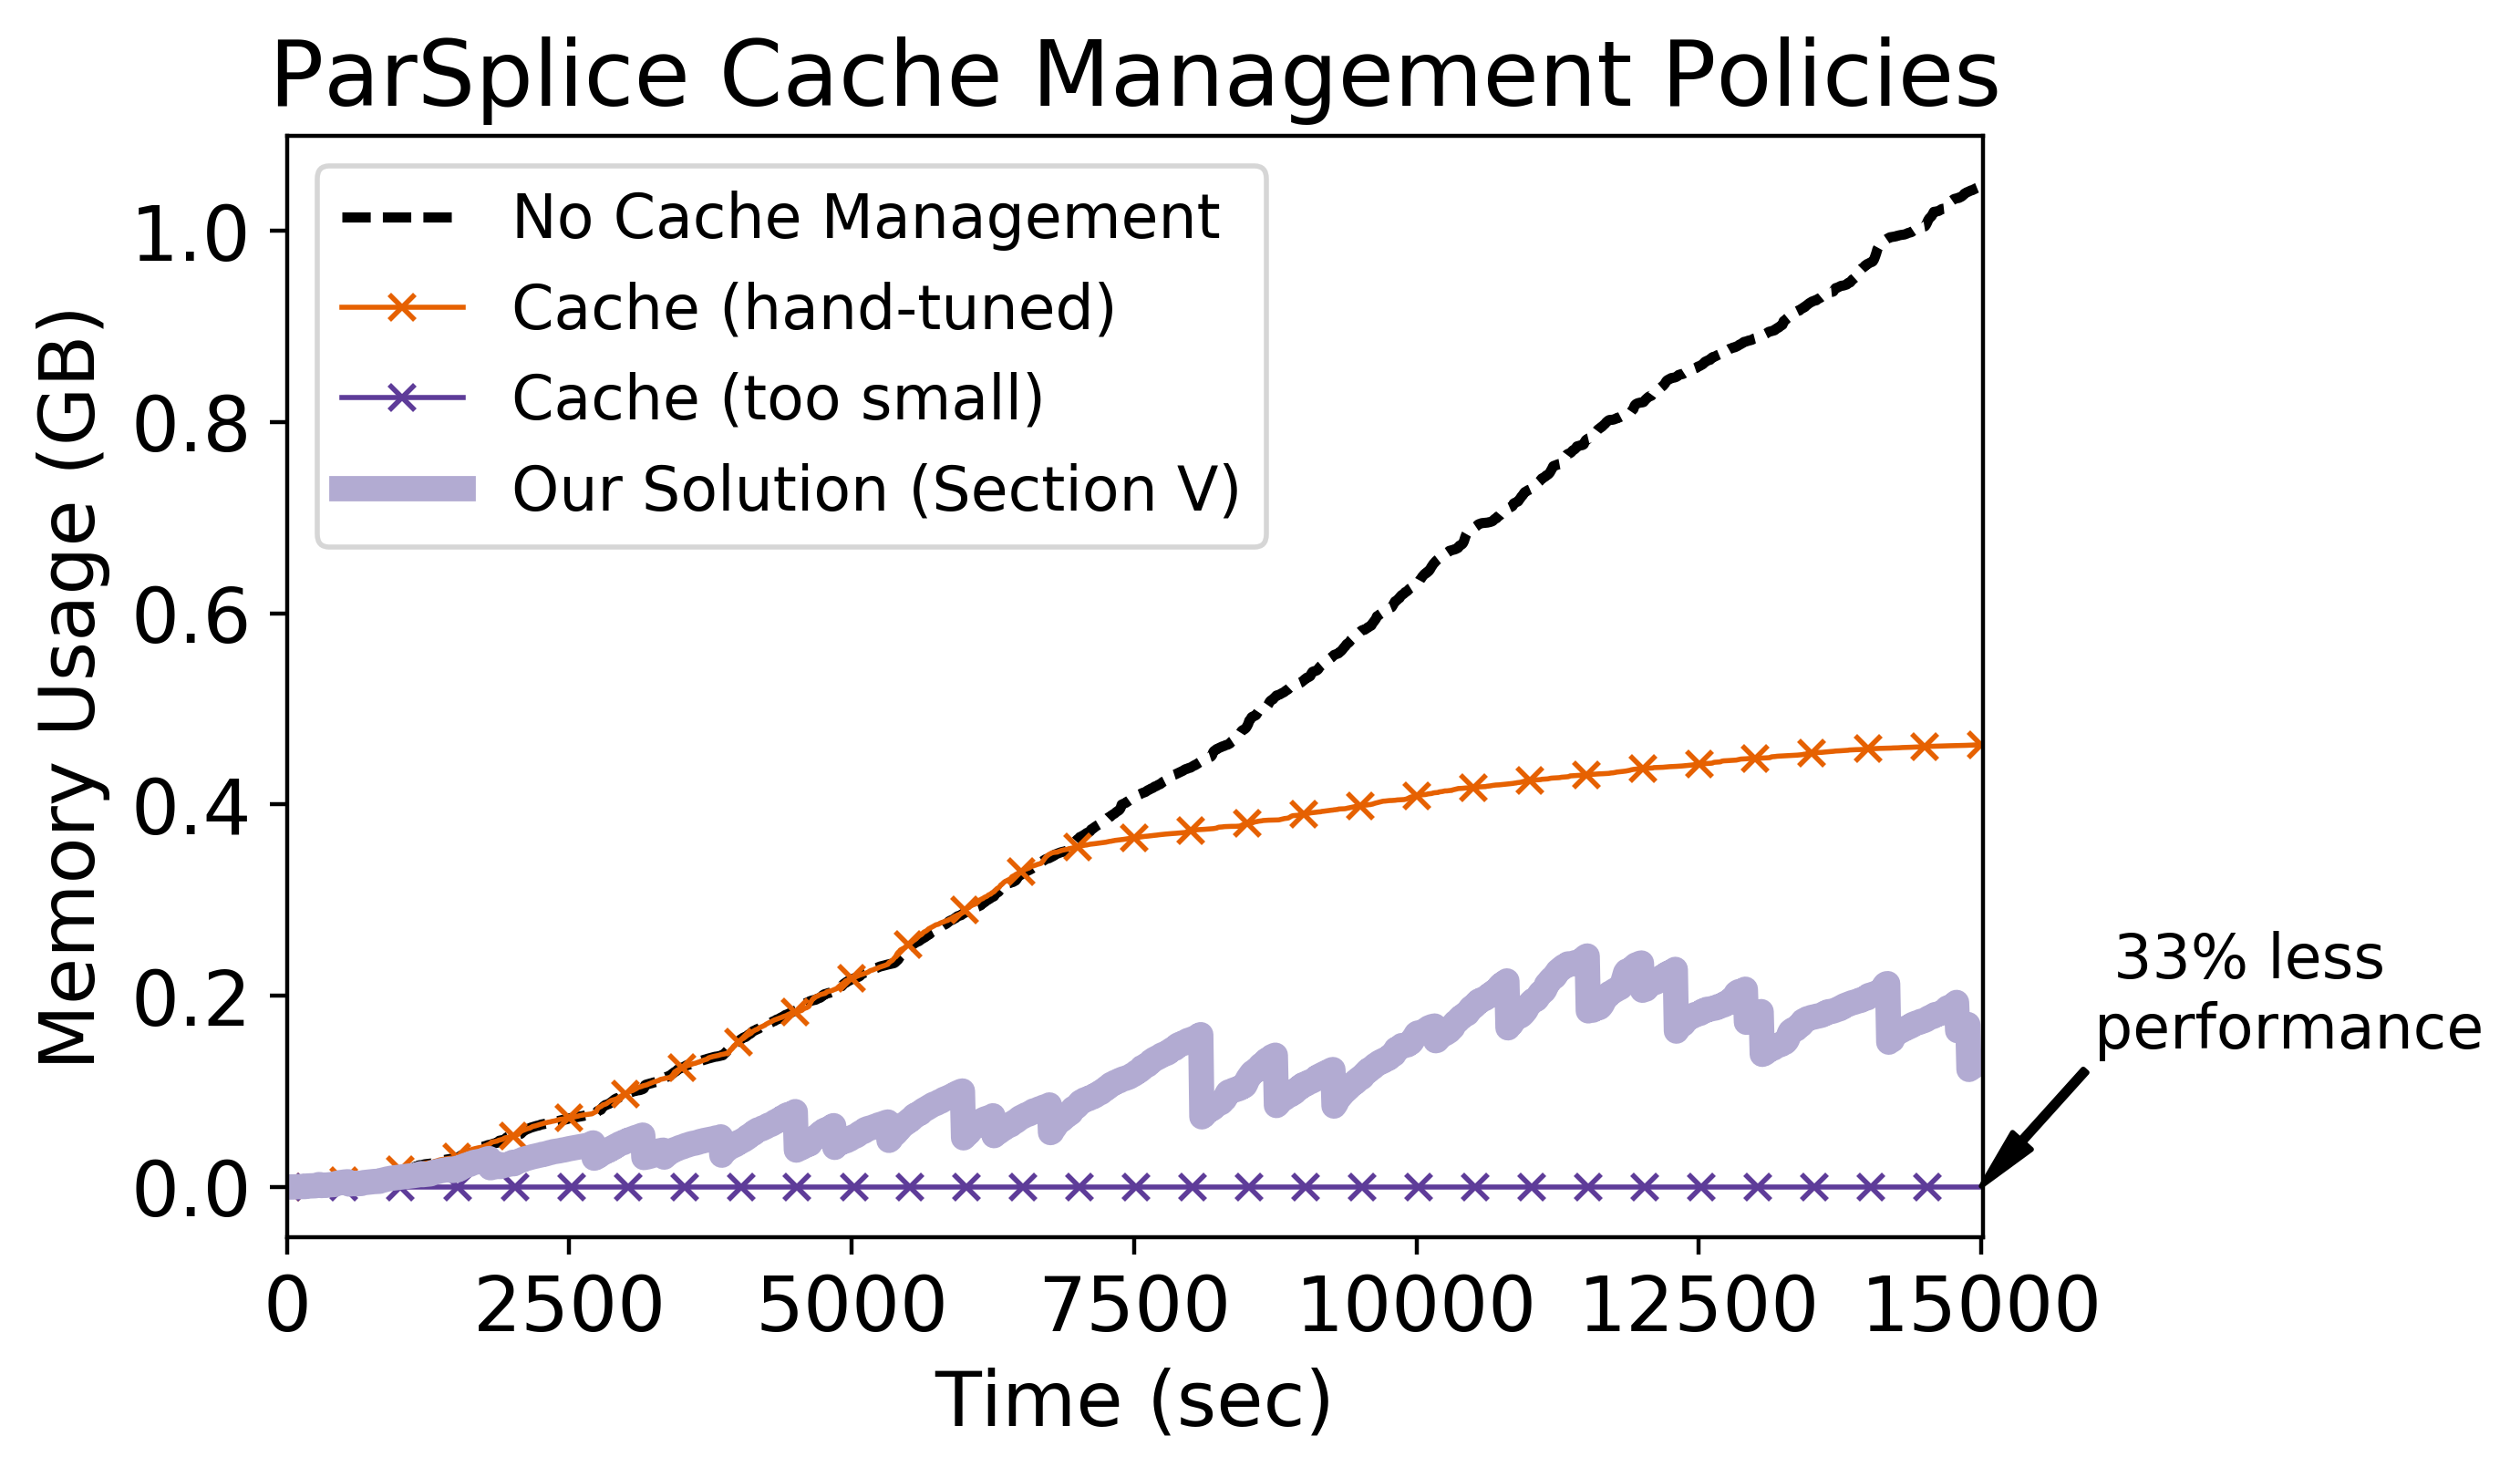
\includegraphics[width=0.5\textwidth]{figures/cache-management.png}\\
\caption{Using our data management language and policy engine, we design a
dynamically sized caching policy (thick line) for ParSplice.  Compared to
existing configurations (thin lines with \(\times\)'s), our solution saves the most
memory without sacrificing performance and works for a variety of inputs.
\label{fig:cache-management}}
\end{figure}

The biggest challenge for ParSplice is properly sizing the caches in the
storage hierarchy.  The memory usage for a single cache that stores molecule
coordinates is shown in Figure~\ref{fig:cache-management}, where the thin solid
lines marked with \(\times\)'s are the existing configurations in ParSplice.
The default configuration uses an unlimited sized cache, shown by the ``No
Cache Management" line, but using this much memory for one cache is
unacceptable for HPC environments, where a common goal is to keep memory for
such data structures below 3\%\footnote{Anecdotally, this threshold works well
for HPC applications.  For reference, a 1GB cache for a distributed file system
is too large in LANL deployments.}. Furthermore, ParSplice deploys a cache per
300 worker processes, so large simulations need more caches and will use even
more memory.  Users can configure ParSplice to evict data when the cache
reaches a threshold but this solution requires tuning and parameter sweeps; the
``Cache (too small)" curve in Figure~\ref{fig:cache-management} shows how a
poorly configured cache can save memory but at the cost of performance, which
is shown by the text annotation to the right.  Even worse, this threshold
changes with different initial configurations and cluster setups so tuning
needs to be done for all system permutations.  Our dynamically sized cache,
shown by the thick line in Figure~\ref{fig:cache-management}, detects key
access patterns and re-sizes the cache accordingly.  Without tuning or
parameter sweeps, our solution saves more memory than a hand-tuned cache
without any performance degradation, works for a variety of initial conditions,
and could generalize to similar applications.

% What is Mantle

In this paper we are presenting the successful use of our data management
language and Mantle policy engine to control the behavior of ParSplice's
caches. Mantle provides a control plane that injects policies into a running
storage system, such as a file system or key-value store. While Mantle was
originally designed for file system metadata load
balancing~\cite{sevilla:sc15-mantle}, we find that it works surprisingly well
for specifying cache management policies without requiring users to possess
extensive knowledge about the internals of storage systems. We show that our
framework:

\begin{itemize}

  \item decomposes cache management into independent policies that can be
  dynamically changed, making the problem more manageable and easier to reason
  about.

  \item can deploy a variety of cache management strategies ranging from basic
  algorithms and heuristics to statistical models and machine learning.

  \item has useful primitives that, while designed for file system metadata
  load balancing, turn out to also be effective for cache management. 

\end{itemize}

% this gives us many policies that are effective across disciplines
% - reuse: eases burden of writing policies
% - autonomic: lays groundwork for an adaptable policy that mixes/matches policies
% FUTURE WORK

This last contribution is explored in Sections~\S\ref{sec:arch-specific}
and~\S\ref{sec:dom-specific}, where we try a range of policies from different
disciplines; but more importantly, in Section~\S\ref{sec:scope}, we conclude
that the collection of policies we design for cache management in ParSplice are
very similar to the policies used to load balance metadata in the Ceph file
system (CephFS~\cite{weil:osdi2006-ceph}) suggesting that there is potential
for automatically adapting and generating policies dynamically.  

%Manageable: abstracts away complexities of the system (pass around to others,
%use different strategies) 

